\documentclass[
  bibliography=totoc,     % Literatur im Inhaltsverzeichnis
  captions=tableheading,  % Tabellenüberschriften
  titlepage=firstiscover, % Titelseite ist Deckblatt
]{scrartcl}
%Bro wir wollen nur was drehen
\usepackage{rotating}
% Paket float verbessern
\usepackage{scrhack}

% Warnung, falls nochmal kompiliert werden muss
\usepackage[aux]{rerunfilecheck}

% unverzichtbare Mathe-Befehle
\usepackage{amsmath}
% viele Mathe-Symbole
\usepackage{amssymb}
% Erweiterungen für amsmath
\usepackage{mathtools}

% Fonteinstellungen
\usepackage{fontspec}
% Latin Modern Fonts werden automatisch geladen
% Alternativ zum Beispiel:
%\setromanfont{Libertinus Serif}
%\setsansfont{Libertinus Sans}
%\setmonofont{Libertinus Mono}

% Wenn man andere Schriftarten gesetzt hat,
% sollte man das Seiten-Layout neu berechnen lassen
\recalctypearea{}

% deutsche Spracheinstellungen
\usepackage[ngerman]{babel}


\usepackage[
  math-style=ISO,    % ┐
  bold-style=ISO,    % │
  sans-style=italic, % │ ISO-Standard folgen
  nabla=upright,     % │
  partial=upright,   % │
  mathrm=sym,        % ┘
  warnings-off={           % ┐
    mathtools-colon,       % │ unnötige Warnungen ausschalten
    mathtools-overbracket, % │
  },                       % ┘
]{unicode-math}

% traditionelle Fonts für Mathematik
\setmathfont{Latin Modern Math}
% Alternativ zum Beispiel:
%\setmathfont{Libertinus Math}

\setmathfont{XITS Math}[range={scr, bfscr}]
\setmathfont{XITS Math}[range={cal, bfcal}, StylisticSet=1]

% Zahlen und Einheiten
\usepackage[
  locale=DE,                   % deutsche Einstellungen
  separate-uncertainty=true,   % immer Unsicherheit mit \pm
  per-mode=symbol-or-fraction, % / in inline math, fraction in display math
]{siunitx}

% chemische Formeln
\usepackage[
  version=4,
  math-greek=default, % ┐ mit unicode-math zusammenarbeiten
  text-greek=default, % ┘
]{mhchem}

% richtige Anführungszeichen
\usepackage[autostyle]{csquotes}

% schöne Brüche im Text
\usepackage{xfrac}

% Standardplatzierung für Floats einstellen
\usepackage{float}
\floatplacement{figure}{htbp}
\floatplacement{table}{htbp}

% Floats innerhalb einer Section halten
\usepackage[
  section, % Floats innerhalb der Section halten
  below,   % unterhalb der Section aber auf der selben Seite ist ok
]{placeins}

% Seite drehen für breite Tabellen: landscape Umgebung
\usepackage{pdflscape}

% Captions schöner machen.
\usepackage[
  labelfont=bf,        % Tabelle x: Abbildung y: ist jetzt fett
  font=small,          % Schrift etwas kleiner als Dokument
  width=0.9\textwidth, % maximale Breite einer Caption schmaler
]{caption}
% subfigure, subtable, subref
\usepackage{subcaption}

% Grafiken können eingebunden werden
\usepackage{graphicx}

% schöne Tabellen
\usepackage{tabularray}
\UseTblrLibrary{booktabs, siunitx}

% Verbesserungen am Schriftbild
\usepackage{microtype}

% Literaturverzeichnis
\usepackage[
  backend=biber,
]{biblatex}
% Quellendatenbank
\addbibresource{lit.bib}
\addbibresource{programme.bib}

% Hyperlinks im Dokument
\usepackage[
  german,
  unicode,        % Unicode in PDF-Attributen erlauben
  pdfusetitle,    % Titel, Autoren und Datum als PDF-Attribute
  pdfcreator={},  % ┐ PDF-Attribute säubern
  pdfproducer={}, % ┘
]{hyperref}
% erweiterte Bookmarks im PDF
\usepackage{bookmark}

% Trennung von Wörtern mit Strichen
\usepackage[shortcuts]{extdash}

\author{%
  Benedikt Nelles\\%
  \href{mailto:authorA@udo.edu}{benedikt.nelles@tu-dortmund.de}%
  \and%
  Tom Bollig\\%
  \href{mailto:authorB@udo.edu}{tom.bollig@tu-dortmund.de}%
}
\publishers{TU Dortmund – Fakultät Physik}

\subject{V408}
\title{Geometrische Optik}
\date{%
  Durchführung: 09.04.2024
  \hspace{3em}
  Abgabe: 15.04.2024
}

\begin{document}

\maketitle
\thispagestyle{empty}
\tableofcontents
\newpage
 

\section{Theorie}
\label{sec:Theorie}

    \noindent Bei Linsen wird generell zwischen Sammellinsen und Zerstreuungslinsen unterschieden. Sammel und Streuungslinsen unterscheiden sich dadrin, dass die Brennweite $f$ bei Sammellinsen positiv ist und bei Zerstreuungslinsen negativ.
    Zusätzlich werden auch zwei Hauptebenen definiert, an denen die Brechung mathematisch modelliert wird. Im Fall einer dünnen Linse fallen die beiden Hauptebenen auf die Mittelebene zusammen. Der Abbildungsmaßstab $V$, der das Verhältnis der Bildgröße $B_g$
    zu der Gegenstandsgröße $G_g$ wiedergibt, wird in diesem Fall auch zu
    \begin{equation}
        V=B_g/G_g=b/g \text{,}
        \label{eqn:abbildung}
    \end{equation}
    \noindent wobei $b$ der Abstand zwischen dem Bild und der Mittelebene ist und $g$ der Abstand vom Gegenstand zur Mittelebene.
    Des weiteren gilt bei solchen Linsen für die Brennweite die Beziehung
    \begin{equation}
        1/f=1/b+1/g \text{,}
        \label{eqn:brenn1}
    \end{equation}
    \noindent wenn das Bild in der Bildebene scharf erscheint.


\cite{sample}

\section{Durchführung}
Bei dem Versuch nimmt eine Kamera Öltropfchen, die eine Dichte von $\rho_{Oel}=\qty{886}{\kilo\gram\per\cubic\meter}$ 
haben, auf, die an einem Gitter, welches Abstände definiert, herunterfließen.
Dabei stehen die Tröpfchen unter dem Einfluss der Gravitation, welche sie immer nach oben zieht,
da das Bild der Kamera invertiert ist, und einem elektrischen Feld, welches nach belieben umgepolt werden kann. 
Des weiteren erfahren die Tröpfchen Reibung am Gitter. Von oben werden dann Öltröpfchen in die Apparatur 
hineingesprüht, zwischen zwei Kondensatorplatten mit einem Abstand von $d=\qty{7.6250(0.0051)}{\milli\meter}$. 
Die angelegte Spannung beträgt hierbei $U_0=\qty{249}{\volt}$. Durch die Umpolung des entstehenden elektrischen
Feldes kann dann die Bewegungsrichtung veräändert werden. Danach wird eine Distanz festgelegt, die das betrachtete
Teilchen zurülegen soll zwischen umpolungen und die Zeit, die das Tröpfchen dann braucht, gemessen. Für jedes Tröpfchen
wird dies mehrmals wiederholt. Desweiteren wurde die Raumtemparatur eines Temparaturempfindlichen
Widerstandes gemessen, woraus sich für die Viskosität der Luft ein Wert von $\eta=\qty{1.834e-5}{\newton\second\per\meter\squared}$
ergibt. Desweiteren betrug der durchschnittliche Umgebungsdruck an dem Tag in Dortmund $p=\qty{1017}{\hecto\pascal}$ \cite{luftdruck}.
\label{sec:Durchführung}

\section{Auswertung}
\label{sec:Auswertung}

In \ref{tab:Tabelle1}. \ref{tab:Tabelle2} und \ref{tab:Tabelle3} sind die Werte für die gemessnen Sink- und Steigzeiten der 10 Öltröpfchen enthalten.

\begin{table}[http]
  \centering
  \caption{In dieser Tabelle ist die gemessene Sink- und Steigzeit von den ersten vier Öltröpchen eingetragen.}
  \label{tab:Tabelle1}
  \sisetup{table-format=1.1, per-mode=reciprocal}
  \begin{minipage}[t]{0.2\linewidth}
    \begin{tblr}[t]{
      colspec = {S[table-format=1.2] S[table-format=1.2] },
      row{1} = {guard, mode=math},
    }
    \toprule
    t_{sink} \mathbin{/} \unit{\second} & t_{steig} \mathbin{/} \unit{\second}  \\
    \midrule
    1.61  &  1.48 \\
    1.87  &  1.40 \\
    1.13  &  1.57 \\
    1.35  &  1.36 \\
    1.43  &  1.54 \\
    1.15  &  1.38 \\
    1.55  &  1.45 \\

    \bottomrule
  \end{tblr}
\end{minipage}
\hfill
\begin{minipage}[t]{0.2\linewidth}
    \begin{tblr}[t]{
      colspec = {S[table-format=1.2] S[table-format=1.2] },
      row{1} = {guard, mode=math},
    }
    \toprule
    t_{sink} \mathbin{/} \unit{\second} & t_{steig} \mathbin{/} \unit{\second}  \\
    \midrule
    2.28  &  2.37 \\
    2.43  &  2.41 \\
    2.21  &  2.40 \\
    2.65  &  2.06 \\
    2.44  &  2.73 \\
    \bottomrule
  \end{tblr}
\end{minipage}
\hfill
\begin{minipage}[t]{0.2\linewidth}
  \begin{tblr}[t]{
    colspec = {S[table-format=1.2] S[table-format=1.2] },
    row{1} = {guard, mode=math},
  }
  \toprule
  t_{sink} \mathbin{/} \unit{\second} & t_{steig} \mathbin{/} \unit{\second}  \\
  \midrule
  2.97  &  2.70 \\
  2.50  &  2.93 \\
  2.42  &  2.66 \\
  2.63  &  2.95 \\
  2.58  &  2.79 \\

  \bottomrule
\end{tblr}
\end{minipage}
\hfill
\begin{minipage}[t]{0.2\linewidth}
    \begin{tblr}[t]{
      colspec = {S[table-format=1.2] S[table-format=1.2] },
      row{1} = {guard, mode=math},
    }
    \toprule
    t_{sink} \mathbin{/} \unit{\second} & t_{steig} \mathbin{/} \unit{\second}  \\
    \midrule
    2.18  &  3.11 \\
    2.70  &  3.03 \\
    3.21  &  2.72 \\
    2.55  &  3.10 \\
    2.44  &  2.89 \\
    \bottomrule
  \end{tblr}
\end{minipage}
\end{table}

\begin{table}[http]
  \centering
  \caption{Hier ist die Sink- und Steigzeit von den Öltröpchen 5 bis 7 eingetragen.}
  \label{tab:Tabelle2}
  \sisetup{table-format=1.1, per-mode=reciprocal}
  \begin{minipage}[t]{0.3\linewidth}
    \begin{tblr}[t]{
      colspec = {S[table-format=1.2] S[table-format=1.2] },
      row{1} = {guard, mode=math},
    }
    \toprule
    t_{sink} \mathbin{/} \unit{\second} & t_{steig} \mathbin{/} \unit{\second}  \\
    \midrule
    3.59  &  4.64 \\
    3.62  &  4.93 \\
    3.74  &  4.61 \\
    3.73  &  4.96 \\
    3.88  &  4.63 \\

    \bottomrule
  \end{tblr}
\end{minipage}
\hfill
\begin{minipage}[t]{0.3\linewidth}
    \begin{tblr}[t]{
      colspec = {S[table-format=1.2] S[table-format=1.2] },
      row{1} = {guard, mode=math},
    }
    \toprule
    t_{sink} \mathbin{/} \unit{\second} & t_{steig} \mathbin{/} \unit{\second}  \\
    \midrule
    2.26  &  2.98 \\
    2.45  &  3.31 \\
    2.34  &  3.16 \\
    2.39  &  2.83 \\
    2.40  &  3.55 \\
    \bottomrule
  \end{tblr}
\end{minipage}
\hfill
\begin{minipage}[t]{0.3\linewidth}
  \begin{tblr}[t]{
    colspec = {S[table-format=1.2] S[table-format=1.2] },
    row{1} = {guard, mode=math},
  }
  \toprule
  t_{sink} \mathbin{/} \unit{\second} & t_{steig} \mathbin{/} \unit{\second}  \\
  \midrule
  4.73  &  4.98 \\
  4.91  &  4.86 \\
  4.56  &  5.69 \\
  4.39  &  6.72 \\
  4.82  &  5.38 \\

  \bottomrule
\end{tblr}
\end{minipage}
\end{table}


\begin{table}[http]
  \centering
  \caption{In der Tabelle ist die gemessene Sink- und Steigzeit von den letzten drei Öltröpchen aufgeführt.}
  \label{tab:Tabelle3}
  \sisetup{table-format=1.1, per-mode=reciprocal}
  \begin{minipage}[t]{0.3\linewidth}
    \begin{tblr}[t]{
      colspec = {S[table-format=1.2] S[table-format=1.2] },
      row{1} = {guard, mode=math},
    }
    \toprule
    t_{sink} \mathbin{/} \unit{\second} & t_{steig} \mathbin{/} \unit{\second}  \\
    \midrule
    4.35  &  8.69 \\
    5.90  &  7.87 \\
    5.99  &  8.48 \\
    5.62  &  7.72 \\
    5.89  &  6.64 \\

    \bottomrule
  \end{tblr}
\end{minipage}
\hfill
\begin{minipage}[t]{0.3\linewidth}
    \begin{tblr}[t]{
      colspec = {S[table-format=1.2] S[table-format=1.2] },
      row{1} = {guard, mode=math},
    }
    \toprule
    t_{sink} \mathbin{/} \unit{\second} & t_{steig} \mathbin{/} \unit{\second}  \\
    \midrule
    3.19  &  4.55 \\
    3.86  &  4.48 \\
    3.63  &  4.31 \\
    3.71  &  4.39 \\
    3.96  &  4.65 \\
    \bottomrule
  \end{tblr}
\end{minipage}
\hfill
\begin{minipage}[t]{0.3\linewidth}
  \begin{tblr}[t]{
    colspec = {S[table-format=1.2] S[table-format=2.2] },
    row{1} = {guard, mode=math},
  }
  \toprule
  t_{sink} \mathbin{/} \unit{\second} & t_{steig} \mathbin{/} \unit{\second}  \\
  \midrule
  6.11  &   8.74 \\
  7.73  &   9.92 \\
  6.84  &   9.79 \\
  7.26  &   9.99 \\
  6.44  &  11.22 \\

  \bottomrule
\end{tblr}
\end{minipage}
\end{table}

Mit der Formel 
\begin{equation*}
  \bar{t}=\frac{1}{n} \sum_{i=1}^n t_i
\end{equation*}
wird der Mittelwert der Sink- und Steigzeiten ausgerechnet und in \ref{tab:Mittelwerte} eingetragen.
Dazu werden auch die Standardabweichungen, berechnet mit 
\begin{equation*}  
  s=\sqrt{\frac{1}{N-1} \sum_{i=1}^N (t_i-\bar{t})^2}
\end{equation*}
berechnet.

\begin{table}[H]
  \centering
  \caption{Aufgeführt sind die Mittelwerte der Sinkzeiten, sowie die entsprechenden Mittelwerte der Steigzeiten mit deren Fehlern.}
  \label{tab:Mittelwerte}
  \sisetup{table-format=1.1, per-mode=reciprocal}
    \begin{tblr}[t]{
      colspec = {S[table-format=2.0] S[table-format=1.3] S[table-format=1.3] S[table-format=1.3] S[table-format=1.3] },
      row{1} = {guard, mode=math},
      vline{2}={2}{-}{text=\clap{$\pm$}},
      vline{4}={2}{-}{text=\clap{$\pm$}},
    }
    \toprule
    N& t_{sink} \mathbin{/} \unit{\second} & & t_{steig} \mathbin{/} \unit{\second} &  \\
    \midrule
    1& 1.441 & 0.243 &   1.454  & 0.074 \\
    2& 2.402 & 0.152 &   2.394  & 0.212\\
    3& 2.620 & 0.189 &   2.806  & 0.117\\
    4& 2.616 & 0.342 &   2.970  & 0.148\\
    5& 3.712 & 0.103 &   4.754  & 0.156\\
    6& 2.368 & 0.064 &   3.166  & 0.251\\
    7& 4.682 & 0.186 &   5.526  & 0.665\\
    8& 5.550 & 0.612 &   7.880  & 0.718\\
    9& 3.670 & 0.266 &   4.476  & 0.119\\
   10& 6.876 & 0.575 &   9.932  & 0.788\\
    \bottomrule
  \end{tblr}
\end{table}

Da $d=\qty{7.6250(0.0051)}{\milli\meter}$ bekannt ist, kann die Geschwindigkeit $v$ der einzelnen Öltröpfchen mit 
\begin{equation}
  v=\frac{s}{t}
\end{equation}
berechnet werden. 
Diese wurden in die Tabelle \ref{tab:Geschwindigkeiten} eingetragen.


\begin{table}[H]
  \centering
  \caption{Hier sind die Geschwindigkeiten der Öltropfchen eingetragen.}
  \label{tab:Geschwindigkeiten}
  \sisetup{table-format=1.1, per-mode=reciprocal}
    \begin{tblr}[t]{
      colspec = {S[table-format=2.0] S[table-format=1.3] S[table-format=1.3] S[table-format=1.3] S[table-format=1.3] },
      row{1} = {guard, mode=math},
      vline{2}={2}{-}{text=\clap{$\pm$}},
      vline{4}={2}{-}{text=\clap{$\pm$}},
    }
    \toprule
    N &v_{sink} \mathbin{/} \unit{\meter\per\milli\second} & & v_{steig} \mathbin{/}  \unit{\meter\per\milli\second}&  \\
    \midrule
    1  & 0.360 & 0.060 & 0.345 & 0.017 \\
    2  & 0.209 & 0.013 & 0.211 & 0.019 \\ 
    3  & 0.192 & 0.013 & 0.179 & 0.007 \\ 
    4  & 0.194 & 0.024 & 0.169 & 0.009 \\ 
    5  & 0.135 & 0.004 & 0.105 & 0.003 \\
    6  & 0.211 & 0.006 & 0.159 & 0.013 \\ 
    7  & 0.107 & 0.004 & 0.092 & 0.010 \\
    8  & 0.091 & 0.012 & 0.064 & 0.006 \\ 
    9  & 0.137 & 0.011 & 0.112 & 0.003 \\ 
   10  & 0.073 & 0.006 & 0.051 & 0.004 \\
    \bottomrule
  \end{tblr}
\end{table}

\section{Diskussion}
\label{sec:Diskussion}
\subsection{Brennweitenbestimmung durch Messung von Gegenstands- und Bildweite}
Mithilfe der Abweichung die in \ref{tab:brenn} berechnet wurden ist erkennbar, dass diese mit steigender Gegenstandsweite auch größer wird.

\noindent Bei der Bestimmung der Brennweite ist das Ergebnis $f \bar=\qty{10.178(0.335)}{\centi\meter}$. 
Die Abweichung dieses Ergebnisses von Theoriewert beträgt mit 
\begin{equation}
    A=\frac{E-T}{T} \cdot \qty{100}{\percent}
    \label{eqn:Abweichung}
\end{equation}
$A_f=\qty{1.8(3.3)}{\percent}$.
Mögliche Fehlerquellen sind hier Messfehler bei der Bestimmung der Gegenstands- und Bildweite, sowie Abweichungen bei der tatsächlichen Brennweite der Linse.

\noindent Die Graphisch bestimmten werte sind $f_{g_1}=x=\qty{9(1)}{\centi\meter}$ und $f_{g_2}=y=\qty{11(1)}{\centi\meter}$ befindet.
Da diese Beiden Werte nich identisch sind, liegt ein Fehler vor.
Für die einzelnen Werte ergeben sich mit Formel \ref{eqn:Abweichung} die Abweichungen $A_{fg1}=\qty{-10(10)}{\percent}$ und $A_{fg2}=\qty{10(10)}{\percent}$
Dieser lässt sich in den zuvor genannten Fehlerquellen begründen, sowie dem Ablesefehler, der beim Ablesen von der Abbildung noch dazu kommt.

\subsection{Brennweitenbestimmung mit der Methode von Bessel}
Der durch diese Methode bestimmte Wert für die Brennweite ist $f_{B}=\qty{9.80(0.06)}{\centi\meter}$.
Bei diesem beträgt die Abweichung zum Theoriewert $A_{f_B}=\qty{2.0(0.6)}{\percent}$.
Die gemessenen Brennweiten mit Farbfiltern sind $f_b=\qty{9.75(0.06)}{\centi\meter}$ und $f_r=\qty{9.82(0.08)}{\centi\meter}$.
Dazu sind $A_{f_Bb}=\qty{-2.5(0.6)}{\percent}$ und $A_{f_Br}=\qty{-1.8(0.8)}{\percent}$ die entsprechenden Abweichungen zum Theoriewert.
Es ist erkennbar, dass Die Brennweite mit blauem Filter niedriger ist, als die ohne Filter.
Zudem ist die Brennweite mit rotem Filter höher, als bei der Messung ohne Filter.
Dieses Ergebnis wird auch so durch chromatische Abberration vorausgesagt.
Jedoch ist durch die Fehler, die sich in derselben Größenordnung wie die Abweichung zu dem Filterlosen Licht befinden, fraglich, inwiefern das Ergebnis wirklich die chromatische Abberration belegt.


\subsection{Brennweitenbestimmung mit der Methode von Abbe}
Die Brennweite, die sich durch die Methode von Abbe für das Linsensystem ergibt, ist $f_A=\qty{20.5(1.0)}{\centi\meter}$.
Dies ist insofern zu erwarten, dass die Brennweite des Linsensystems größer ist, als die der einzelnen Sammellinse mit $f=\qty{10}{\centi\meter}$,
da das Licht nun gestreut wird, bevor es die Sammellinse erreicht und sich dadurch der Brennpunkt nach hinten verschiebt.
Berechnet wurde ein Wert von $f_{A_t}=\qty{22.22}{\centi\meter}$ und die mit Formel \ref{eqn:Abweichung} ausgerechnete Abweichung beträgt $A_{f_A}=\qty{-8(5)}{\percent}$.
Dies könnte, neben möglichen Fehlern während der Messung, auch durch die Näherungen bei der theoretischen Berechnung kommen.
In dieser wird nämlich sphärische Abberation nicht berücksichtigt.


\printbibliography{}

\section{Anhang}

\begin{figure}[H]
  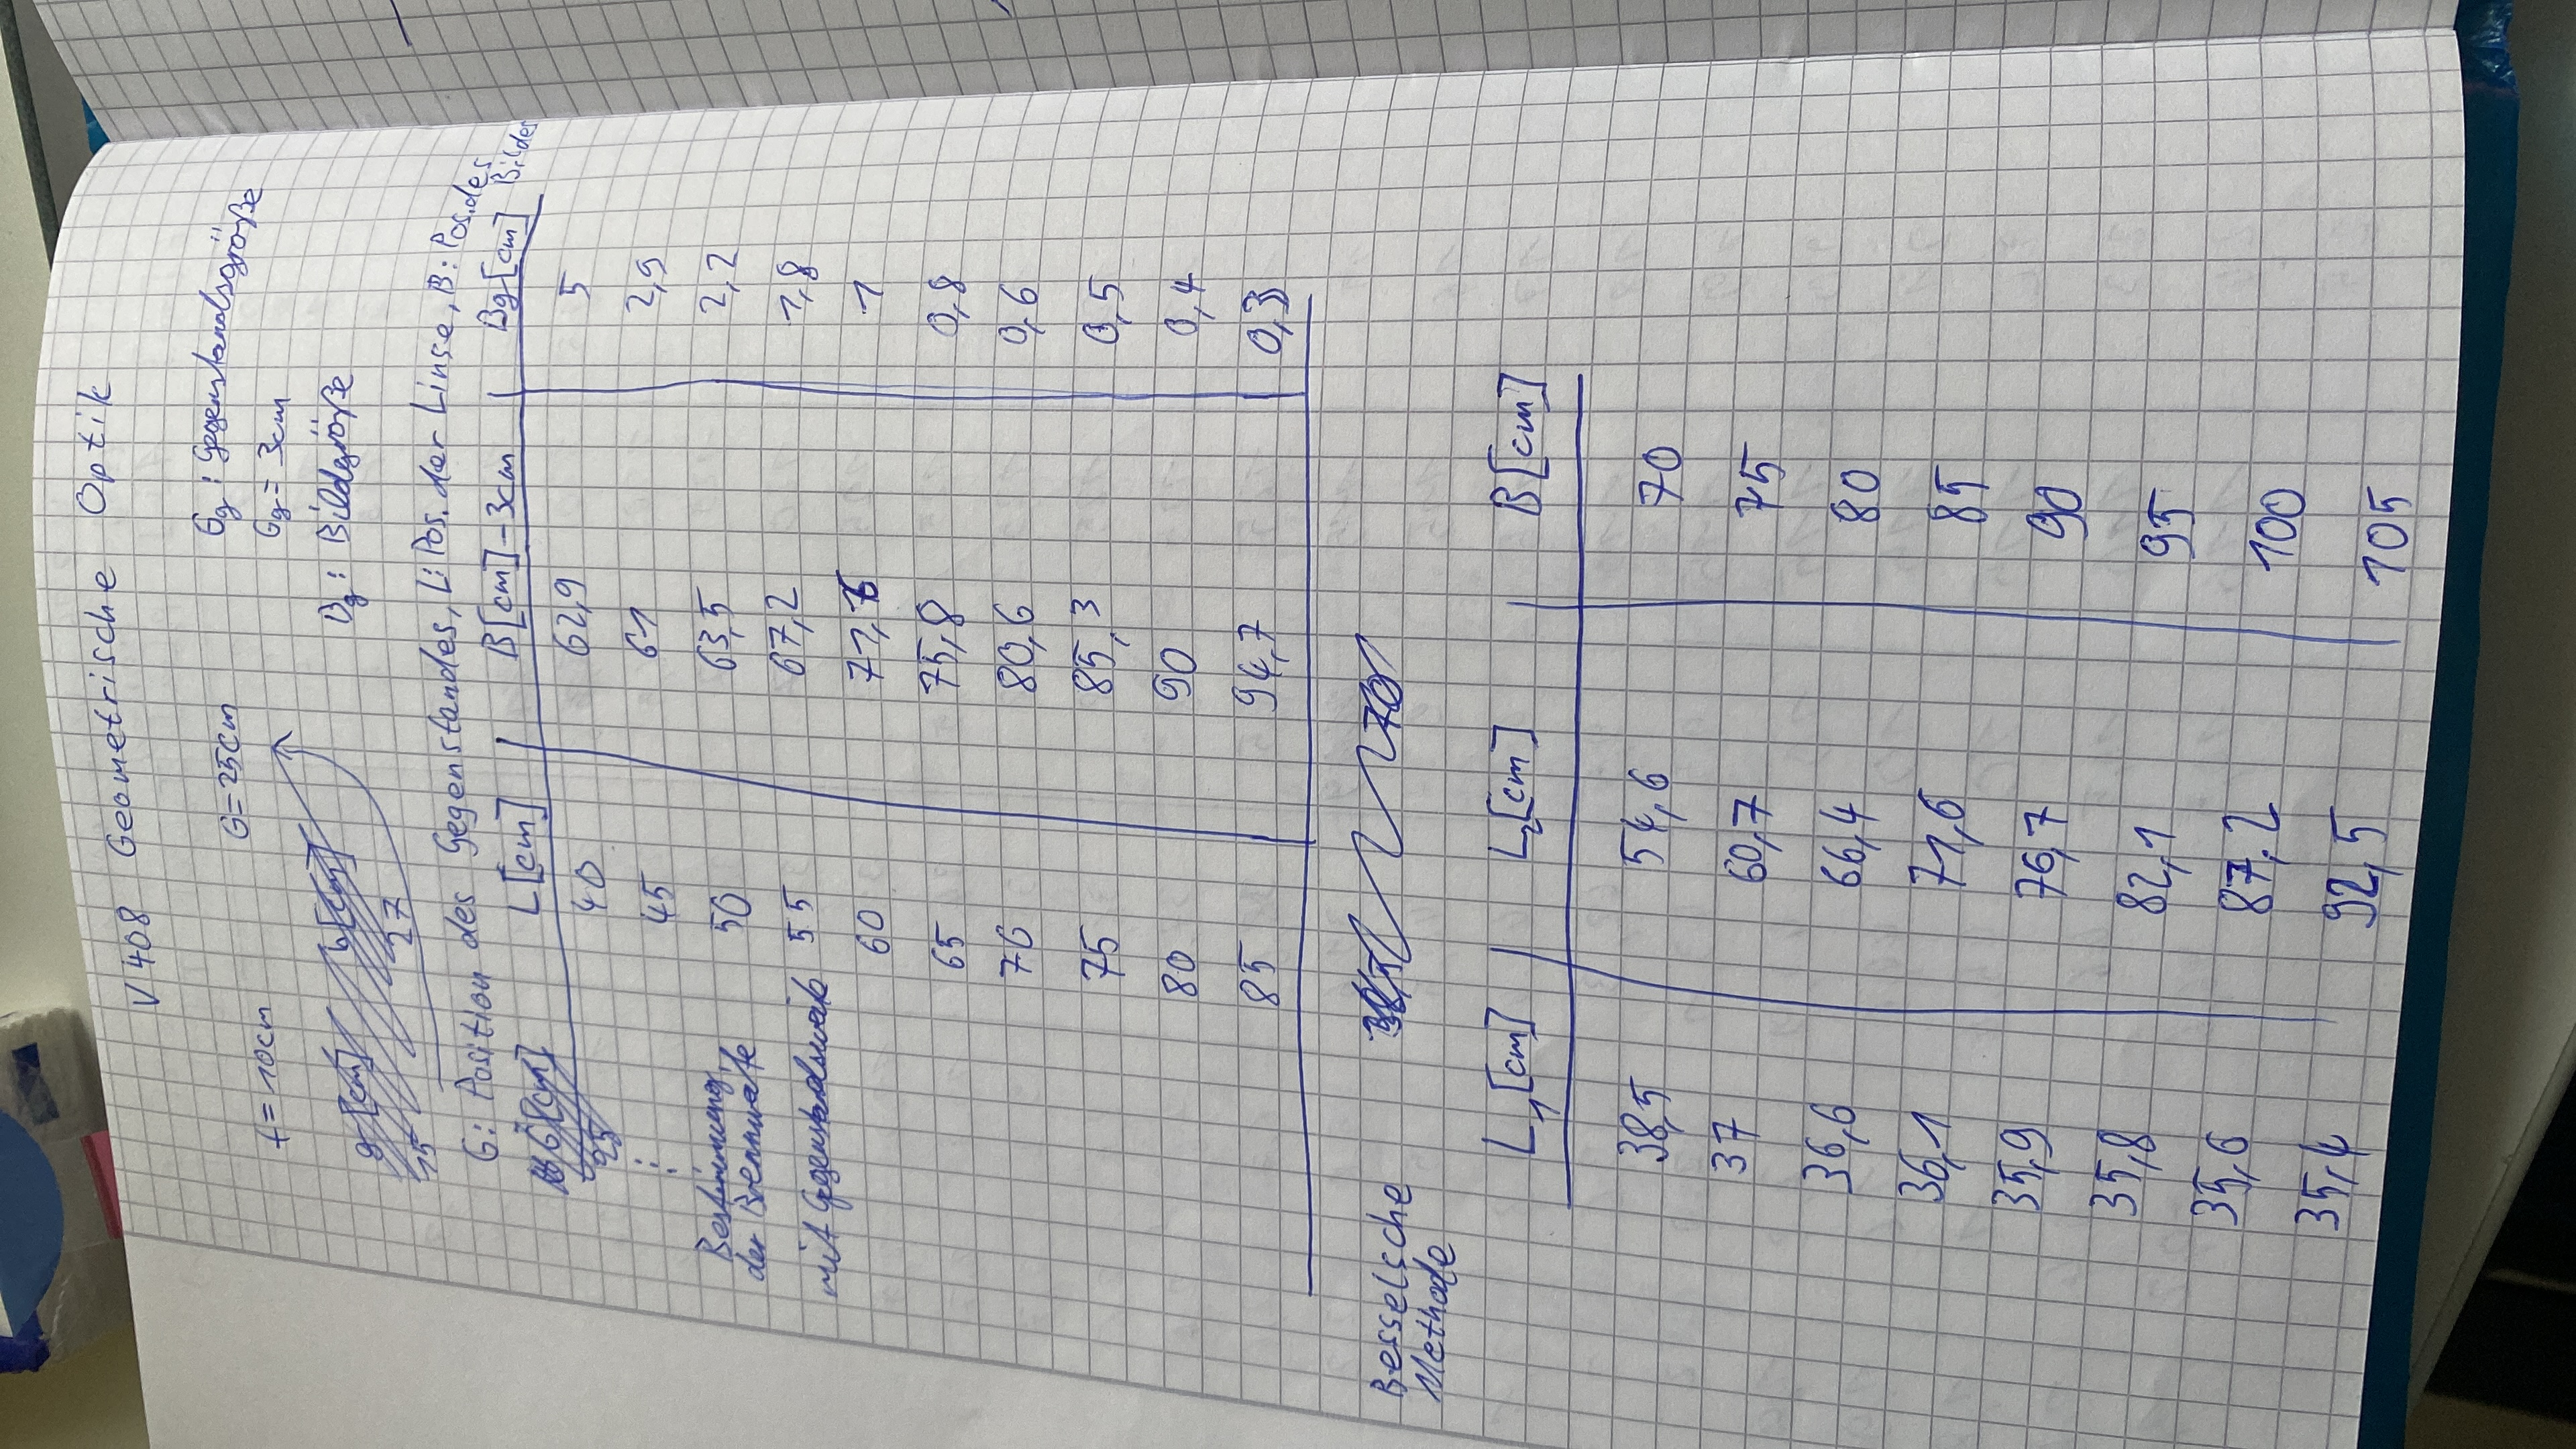
\includegraphics[width=\textwidth, height=15cm, angle=270]{Bilder/Messdaten1.JPG}
  \caption{Rohdaten 1}
\end{figure}

\begin{figure}[H]
  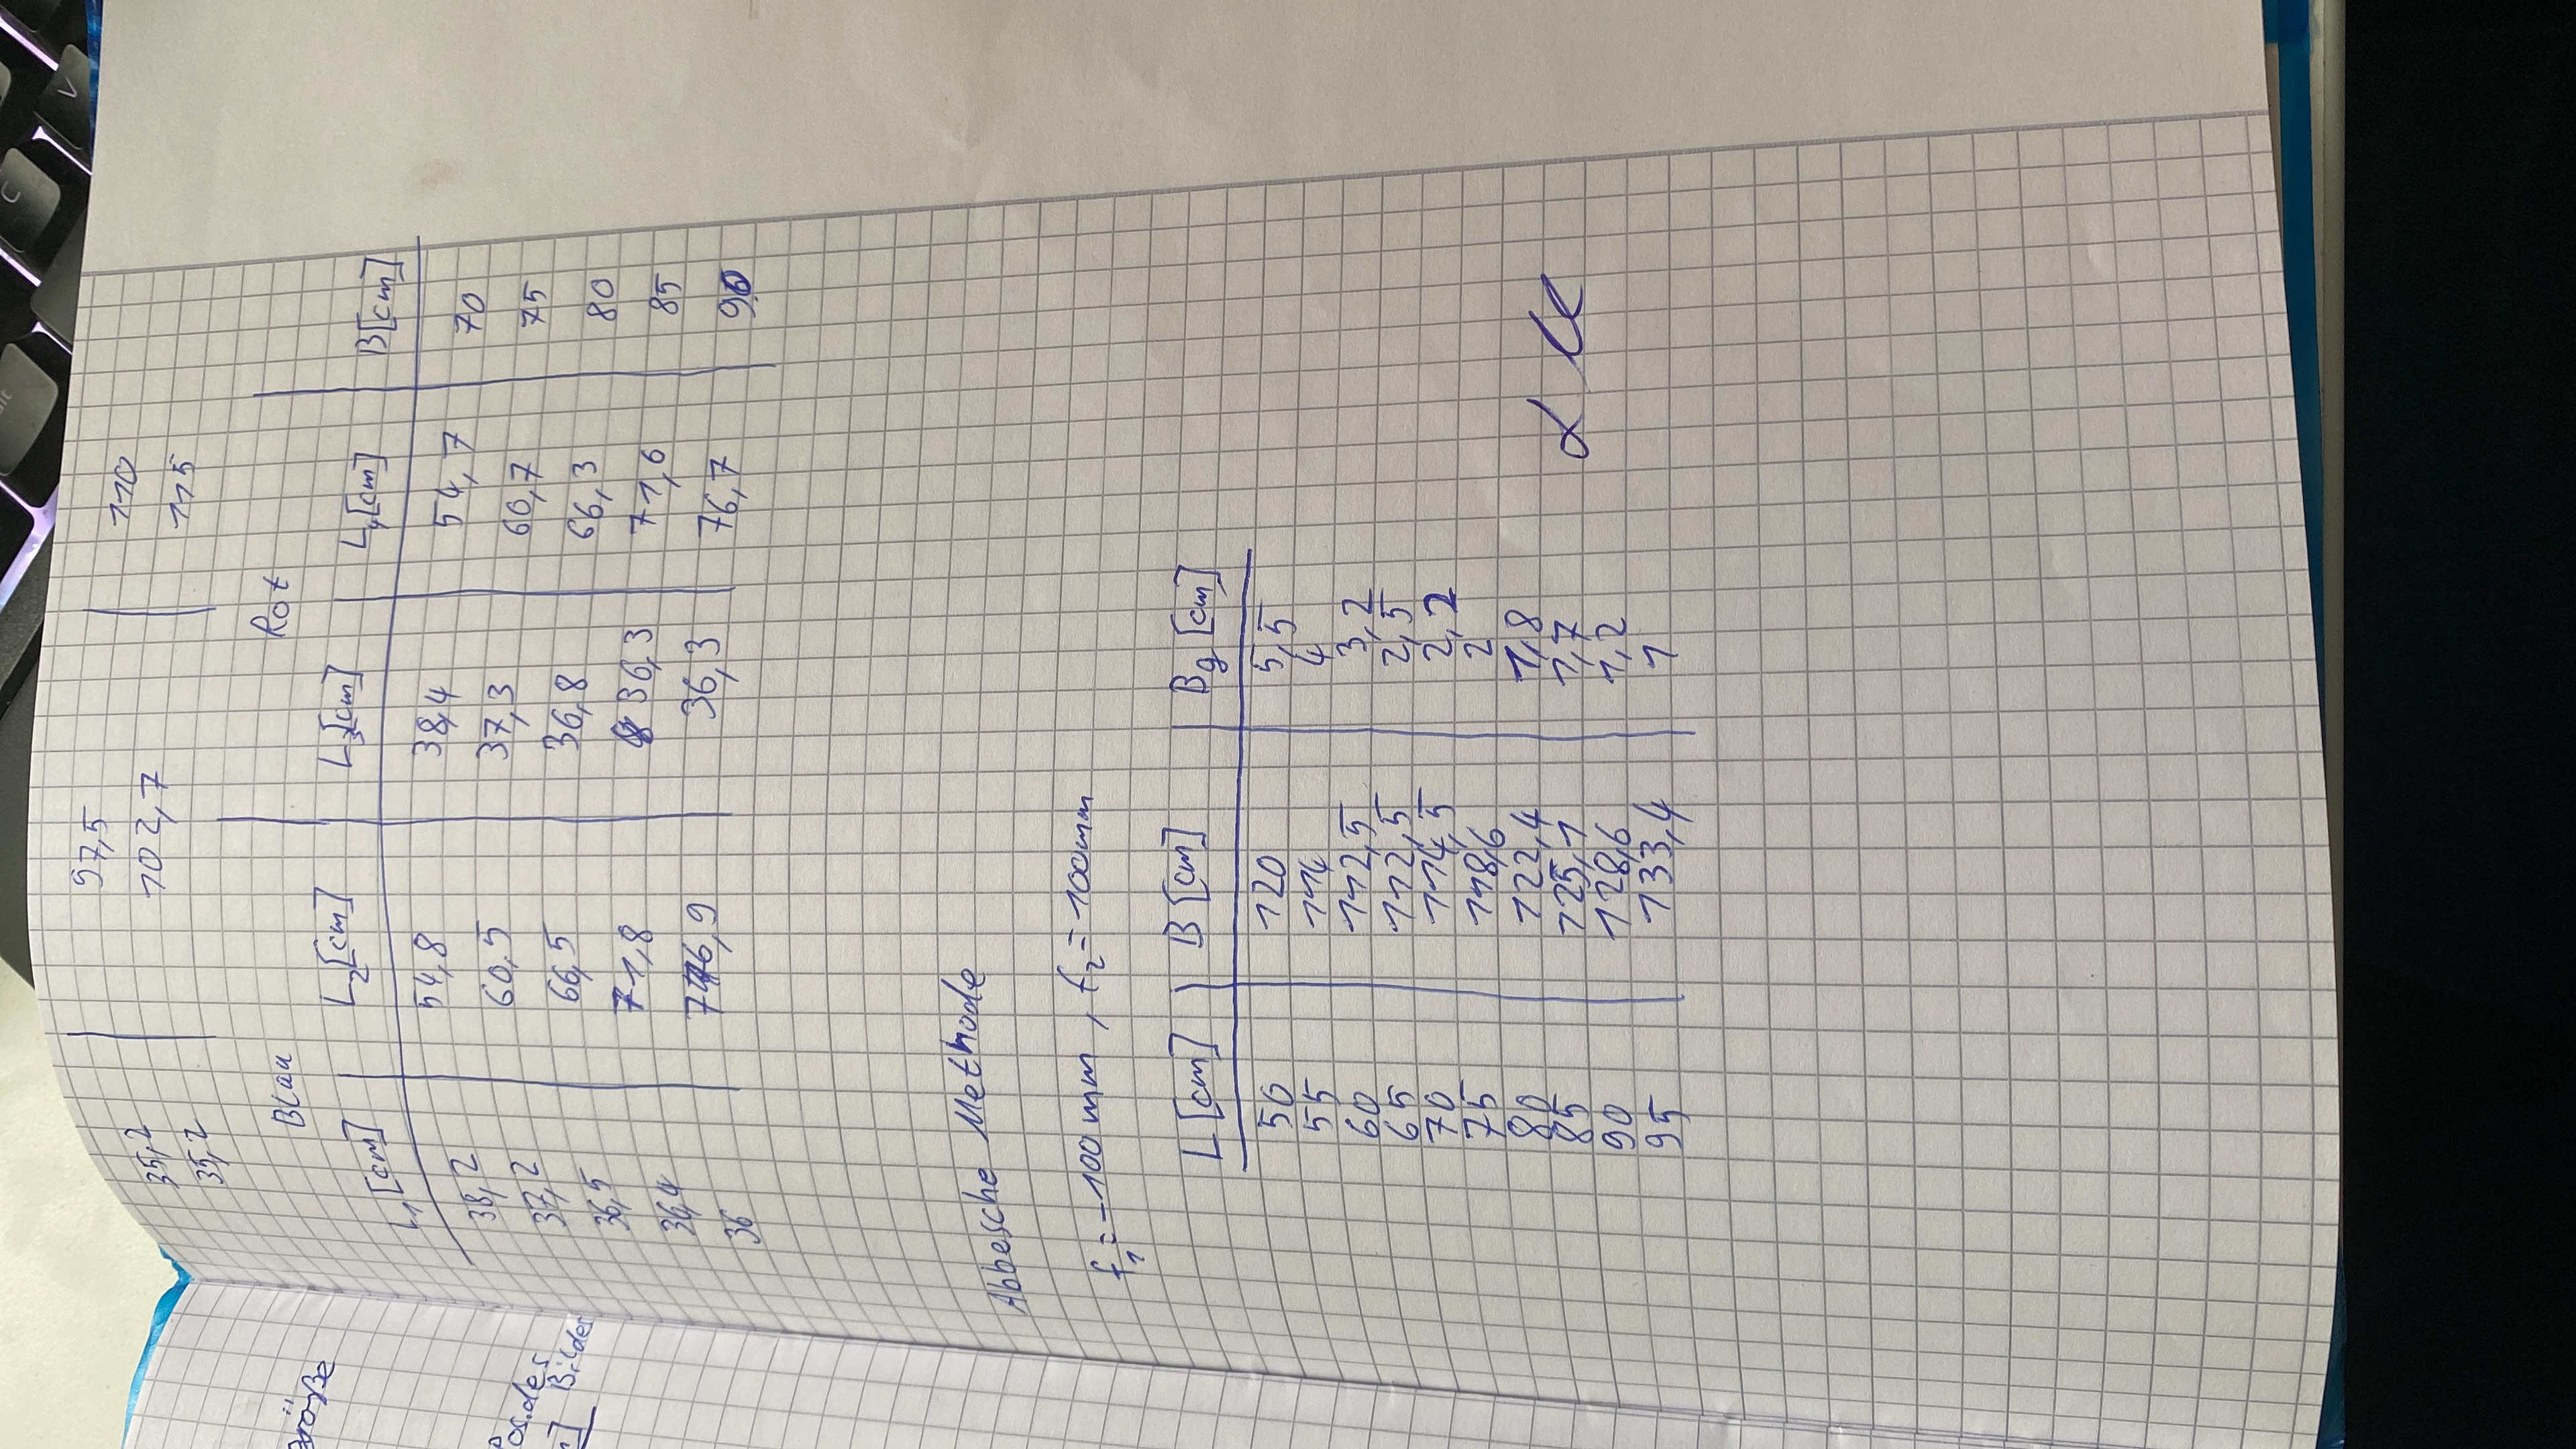
\includegraphics[width=\textwidth, height=15cm, angle=270]{Bilder/Messdaten2.JPG}
  \caption{Rohdaten 2}
\end{figure}


\end{document}
